\documentclass{l4proj}

\usepackage{url}
\usepackage{fancyvrb}
\usepackage[final]{pdfpages}
\usepackage{hyperref}
\usepackage{fancyvrb}
\usepackage{float}
\usepackage{multirow}
\usepackage{graphicx}
\usepackage{amsmath}
\usepackage{MnSymbol}
\usepackage{wasysym}


\hypersetup{
    colorlinks,
    citecolor=black,
    filecolor=black,
    linkcolor=black,
    urlcolor=black
}

\begin{document}
\title{Implementations of Advanced K-Means Clustering Algorithms \\ for Spark/MLlib}
\author{Ivan Kyosev}
\date{March 21, 2017}
\maketitle

\begin{abstract}
Apache Spark is a fast and general engine for large-scale data processing. It emphasizes speed, ease of use and generality in regards to working with Big Data. Its feature-set provides an alternative to the popular Hadoop MapReduce software framework, displaying a noticeable performance improvement. One of Spark's many components is MLlib. It is a machine learning library built on top of the core features of Spark and provides implementations for a variety of popular machine learning algorithms, written in a way meant to support scalability when operating on big data sets.

This paper presents a proposed extension to the MLlib component of Apache Spark in the form of additional K-Means Clustering algorithms that the library does not currently support. K-Means clustering is a method of vector quantization, originally from signal processing, that is popular for cluster analysis in data mining. A thorough analysis of the performance of the newly created algorithms and the relative quality of the produced data models is also conducted.
\end{abstract}

\educationalconsent

\tableofcontents

\chapter{Introduction}
\label{intro}
\pagenumbering{arabic}

Machine learning is an increasingly popular and relevant part of modern day systems looking to extract knowledge and value from the world around them. It refers to an approach to computation, where applications can learn without being explicitly programmed. These kinds of apps can analyze a provided sample of data and make predictions or decisions, based on some form of discovered pattern or correlation between the individual elements of the input set.

By being able to take rational choices, through examining the surrounding environment, systems that employ machine learning have become a central component of artificial intelligence. Because these system adapt their behavior based on new ``experiences'' they are utilized in a wide range of computing tasks, where developing explicit algorithms is not feasible. Such examples include solving problems in speech recognition, vision and robotics.

These machine learning algorithms are typically classified into three different categories based on the nature of the data they are learning from and the feedback of information for each input item:

\begin{itemize}
\item Supervised learning - in this case a program presented with a particular input set of data is also provided with the desired output, with the end goal of having the machine learn a mapping function from inputs to outputs
\item Unsupervised learning - here the elements of the input data set are not provided with a desired output value in pairs, so the system is left on its own to find structure in its input
\item Reinforcement learning - this refers to the idea of having an program interact with a dynamic environment, where it is attempting to achieve a certain goal. Along with every action, the program is also provided with positive or negative feedback, depending on whether the action aided in achieving the goal or not. 
\end{itemize}

Many of these machine learning algorithms have a similar underlying approach to their implementation. Input training data with some unknown probability distribution is presented and the program has to construct a model that allows it to extract meaning from the data and make sufficiently accurate predictions for instances that have not been encountered yet. This is generally achieved by defining a loss function and adjusting the model in attempts to minimize this loss with respect to the inputs -- effectively an optimization problem.

It is clear that machine learning algorithms heavily depend on the availability of input data in order to optimize their models to more accurately reflect the state of the real world. Therefore the quantity of supplied input data begins to have a significant impact on the quality of the output produced by application relying on machine learning. With the advent of big data and technologies meant to enable fast and reliable processing of big data, these algorithms can now make use of vast amounts of information, enabling them to create more accurate and valuable results. Examples of big data processing frameworks include Hadoop and Apache Spark.

The Apache Spark project in particular includes a component called MLlib. MLlib is a machine learning library built on top of the core features of Spark. It provides implementations for a variety of popular machine learning algorithms, all of which are written in a way meant to support horizontal scalability\footnote{Horizontal scaling refers to the scaling of a system by adding more parallel, similar in performance nodes. It is directly contrasted by vertical scaling where additional resources are added to the one node of a system.} when operating on big data sets.

\section{Aims}

The aim of this project is to create an extension to the MLlib component of Apache Spark, by developing implementations for a variety of K-Means clustering algorithms that the framework does not currently support. The newly introduced algorithms also need to be evaluated and contrasted with the ones already provided by Spark.

K-Means clustering is an example of an unsupervised machine learning algorithm. It is a method of vector quantization\footnote{Quantization is the process of mapping a large set of input values to a smaller set.}, that originated from signal processing. Its primary purpose is to group a collection of \texttt{N} data points into \texttt{K} distinct clusters. There is a variety of algorithms that produce the end result of grouping data points into \texttt{K} clusters, with varying levels of speed and accuracy. The ones that this project aims to implement as part of Spark could deliver a desired performance improvement with minimal loss in quality.

\section{Report outline}

The remainder of this report will focus on the mathematics underlying each of the considered K-Means clustering algorithms as well as the challenges of implementing them in a scalable fashion under Spark:
\begin{itemize}
\item \textbf{Chapter~\ref{spark}} covers the data processing model provided by Apache Spark and its machine learning library MLlib
\item \textbf{Chapter~\ref{kmeans}} explains the most common used versions of K-Means Clustering algorithms
\item \textbf{Chapter~\ref{previous}} discusses the approach taken by Spark's developers to create the current clustering API
\item \textbf{Chapter~\ref{propose}} outlines the proposed algorithms to be implemented as part of Apache Sparks, along with their benefits and challenges
\item \textbf{Chapter~\ref{online}} details two different approaches to the implementation of Lloyd's Online K-Means Clustering algorithm
\item \textbf{Chapter~\ref{art}} presents a version of K-Means using Adaptive Resonance Theory and its implementation
\item \textbf{Chapter~\ref{som}} presents the implementation of a  a K-Means Clustering algorithm using Self-Organizing Maps
\item \textbf{Chapter~\ref{eval}} covers a variety of ways to evaluate both the performance of the presented algorithms and the quality of the data models they produce
\item \textbf{Chapter~\ref{conclusion}} Concludes this report with a reflection on the whole project
\end{itemize}

%==============================================================================

\chapter{Introduction to Apache Spark and MLlib}
\label{spark}
\section{Apache Spark}

A new big data processing paradigm in the form of cluster computing has become widely popular in recent years. It is a model where data-parallel computations are executed on clusters of unreliable machines by systems that provide scheduling, fault tolerance and load balancing\cite{Spark}. Hadoop MapReduce was the first software framework to implement these principles\cite{MapReduce}, with systems like Dryad and Map-Reduce-Merge generalizing the supported types of data flows. These system achieve fault tolerance and scalability by supplying the user with a means of expressing computation as an acyclic data flow graph which passes the input data through a set of operations. This enables the underlying system to handle any occurring faults as well as scheduling without any user interaction.

Apache Spark is one of the latest big data processing frameworks which implements the cluster computing model. One of its primary advantages over Hadoop is that it can perform in-memory data processing, while Map-Reduce persists all outputs back to disk after a map or reduce action. This extends the scope of problems which can be solved efficiently by Spark to also include applications that reuse a working set of data across multiple parallel operations. It is impractical to implement these kinds of apps under Hadoop as between each iteration of an algorithm over the working set, the job must reload the data from disk, causing unnecessary overhead, resulting in degraded performance. Examples include iterative jobs and interactive analysis\cite{Spark}.

Due to its differences in design philosophy, users of the Spark framework have reported a 100x speed increase in certain work loads, versus a similar MapReduce solution, as well as a 10x faster execution on disk\cite{webSpark}. This performance improvement, however, results in the system requiring more RAM to carry out its operations.

The core components of Spark are implemented in Scala - a statically typed functional programming language that runs on top of the Java Virtual Machine. It also includes object-oriented features and supports Java interoperability thanks to its JVM roots -- this allows Spark to easily interact with Java based systems such as HDFS. In addition to Scala the framework also export an API available in Java, Python and R.

Spark can also be used interactively from a modified version of the Scala interpreter. This method provides full access to the API, allowing a user to define variables, functions, classes and run parallel jobs on a computer cluster. Spark is possibly the first system that allows a general-purpose programming language to be used interactively to process large data sets on a cluster\cite{Spark}.

\section{Resilient Distributed Datasets}

To achieve its goals, Spark introduces an abstraction called resilient distributed datasets -- RDDs. They are a parallel, fault-tolerant data structure that lets users explicitly persist intermediate results in memory, control their partitioning to optimize data placement, and manipulate them using a rich set of operations\cite{RDD}. The RDD API is the primary way of expressing computation on big data sets in Apache Spark.

\subsection{Basics of the RDD API}

An RDD is a read-only partitioned collection of records. It supports a series of methods that resemble operations, available to most collections in a functional programming language\footnote{Despite the nature of the RDD based API, code written in Spark does not need to adhere to the principles of pure functional programing.}. RDDs can only be created through deterministic operations on either data in stable storage or other RDDS. These kind of functions are known as transformations -- examples include \textit{map}, \textit{filter}, \textit{flatMap} and others. Transformations are lazy\footnote{A lazy function is not evaluated when it is called, but rather when something else tries to access its result.} operations that define a new RDD, which is typically the result of applying the same function to every data item in the source RDD -- making Spark ideal for batch processing. By chaining together several of these transformations a user can define a directed acyclic graph (DAC) of operations the data needs to pass through (achieved in a parallel fashion).

Along with transformations, the RDD API also supports actions. These are operations that return a value to the application or export data to a storage system. Examples of actions include - \textit{count}, \textit{collect}, \textit{reduce} and others. Typically a user would define a DAC of transformations to be performed on some data source, these operations would then not be executed until an action is invoked, at which point the result of all transformations in the DAC is evaluated along with the specified action at the end. If there is a large sequence of transformations within the DAC of an RDD, that will be operated on in the end by multiple different actions (branching towards a later point in the DAC), a developer might choose to checkpoint an intermediate stage of the RDD, so that Spark does not need to recompute every operation applied to that RDD.

\begin{table}[H]
\label{Actions and Transformations}
\caption{Transformations and actions available on RDDs in Spark.}
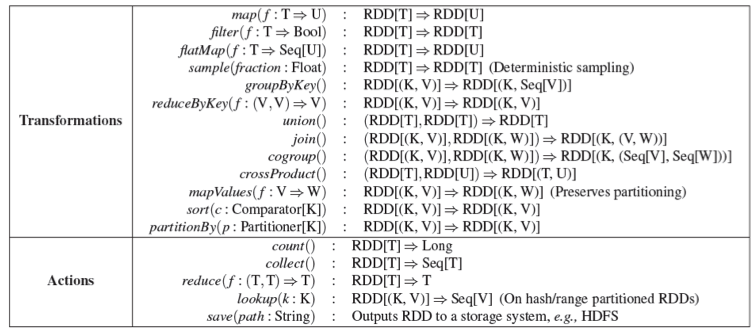
\includegraphics[width=1.0\textwidth]{images/spark-trans-action-edited}
\end{table}

\subsection{RDD fault-tolerance}

To begin the processing of an RDD, the individual data partitions (making up the source used to create the RDD -- typically a file in HDFS), are sent to different nodes in the computing cluster where the user defined DAC of operations is executed simultaneously for each partition (if the system could afford to allocate enough resources for a one-to-one mapping of partitions to cluster nodes). In a large scale distributed system, however, failure of individual hardware components is to be expected. When one of the clusters fails, while processing an RDD partition, Spark is able to reconstruct the lost data without notifying the user.

Because RDDs provide an interface based on transformations (e.g. map, flatMap) that apply the same operations to many data items, they can efficiently provide fault-tolerance by logging the transformations used to build a dataset rather than the actual data (although checkpointing RDDs can have its advantages as previously mentioned). This log of operations is also known as the lineage of the RDD. Thus if a partition of an RDD is lost, the RDD has enough information about how it was derived from other RDDs to recompute just the missing partition\cite{RDD}. Therefore lost data can be quickly recovered without the need for costly replication.

The lineage of an RDD is a powerful property, since it ensures that a program cannot reference an RDD that it cannot reconstruct after failure -- it can always recompute all partitions from data in stable storage.

\subsection{RDD representation}

The Apache Spark framework provides a graph-based representation of RDDs where each dataset has a common interface, exposing five pieces of information:

\begin{itemize}
\renewcommand{\labelitemi}{\scriptsize$\blacksquare$}
\item a set of partitions, which are atomic pieces of the dataset
\item a set of dependencies on parent RDDs
\item a function for computing the dataset based on its parents
\item metadata about its partition scheme
\item metadata about its data placement
\end{itemize}

An RDD representing an HDFS file, for example, has as many partitions as the file has blocks and knows on which machine each block is on. If a map transformation were to be applied on this RDD, the resulting dataset would have the same partitions, but the map function would be applied on the parent's data when computing its elements.

An important aspect of this common interface is the representation of dependencies between RDDs. They are classified into two types: \textit{narrow} dependencies, where each partition of the parent RDD is used by at most one partition of the child RDD, and \textit{wide} dependencies where multiple child partitions may depend on a single parent partition\cite{RDD}. The \textit{map} operation would be an example of a narrow dependency, where as \textit{groupByKey} would result in a wide dependency.

The distinction between these two forms of dependencies has two primary implications. First, narrow dependencies allow for pipelined execution on one cluster node. This means that multiple successive operations resulting in narrow dependencies can be carried out on an RDD partition in the same computing cluster, without needing to move data between cluster nodes. Wide dependencies, however, require that data from all parent partitions to be available and to be shuffled across the nodes of the cluster. Second, narrow dependencies allow for a more efficient recovery from failure, as only the lost partitions need to be recomputed -- this can also be done in parallel on different processing nodes. When there are wide dependencies in the lineage graph of an RDD, however, a single failed node could loose information derived from all parent partitions, requiring a full re-execution of all transformations in the DAC, operating on the RDD.

\begin{figure}[H]
\label{RDD dependencies}
\caption{Examples  of  narrow  and  wide  dependencies.  Each box is an RDD, with partitions shown as shaded rectangles.}
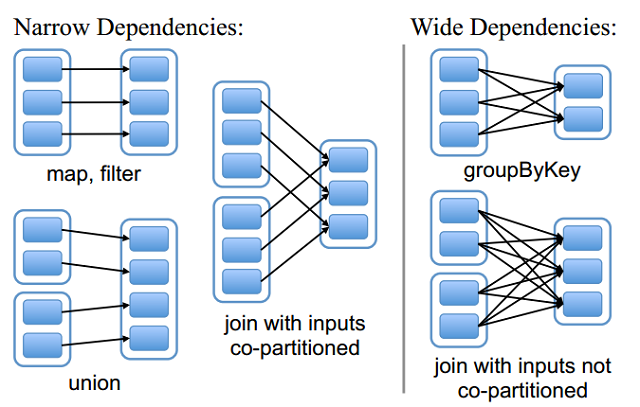
\includegraphics[width=1.0\textwidth]{images/rdd_dependency}
\end{figure}

\section{Shared Variables}

When invoking transformations on an RDD -- such as \textit{map} and \textit{filter}, developers pass closures (functions) to Spark. Similar to functional programming these closures can refer to any variable in the scope where they are created. Once Spark begins the execution of those transformations on a worker node, the referenced local variables are copied to the worker. However, Spark also allows programmers to create two restricted types of shared variables to support common usage patterns\cite{Spark}.

If a Spark program contains a large read-only piece of data that is used in multiple parallel operations, it is preferable to distribute it to the workers only once, as opposed to including it with each closure. This is accomplished by creating a ``broadcast variable'' object which acts as a wrapper for the desired value. It ensures that it is only copied once to each worker, thus reducing network traffic and improving performance.

The second type of shared variables provided by Spark are known as ``accumulators''. Workers can only ``add'' to these variables by using an associative operation, and their value can only be read by the driver program. They enable easy implementations of counters (similar to MapReduce) and provide a more imperative syntax for parallel sums. Accumulators can be defined for any data type that has a ``zero value'' and an ``add'' operation.

\section{Spark Streaming}

TODO: DStreams

\section{MLlib}

TODO: The MLlib paper

%==============================================================================

\chapter{K-Means Clustering}
\label{kmeans}

top level k-means text?

\section{Iterative K-Means Clustering}

iterative k-means text

\section{Mini-batch K-Means Clustering}

mini-batch text

%==============================================================================

\chapter{Previous Work in MLlib}
\label{previous}

\section{Implementation of Iterative K-Means Clustering}

\section{Implementation of Mini-batch K-Means Clustering}

%==============================================================================

\chapter{Proposed Extension to Spark/MLlib}
\label{propose}

\section{Online K-Means}

\section{Adaptive Resonance Theory K-Means}

\section{Self-Organizing Maps K-Means}

\section{Benefits of Online Algorithms}

\section{Implementation Challenge in Parallelizing Sequential Algorithms}

%==============================================================================

\chapter{Online K-Means}
\label{online}

\section{Implementation Using Grand Mean}

\section{Implementation using Spark Streaming}

%==============================================================================

\chapter{Adaptive Resonance Theory K-Means}
\label{art}

\section{Implementation Using Spark Streaming}

%==============================================================================

\chapter{Self-Organizing Maps K-Means}
\label{som}

\section{Implementation Using Spark Streaming}

%==============================================================================

\chapter{Performance Evaluation and Data Model Analysis}
\label{eval}

maybe add an evaluation section earlier to each part\\
add chapter comparing algorithms at the end\\
both would need to explain evaluation method earlier\\
make a reference to the used training data

\section{Sum of Squared Distances}

\section{Silhouette}

%==============================================================================

\chapter{Conclusion}
\label{conclusion}

conclusion text - multiple sections?

%==============================================================================

\bibliographystyle{plain}
\bibliography{l4proj}

%==============================================================================

\begin{appendices}

\chapter{First Appendix}

\end{appendices}

\end{document}